\documentclass[11pt,a4paper]{article}

% ---------- arxiv-style preamble (xelatex; emoji-native) — demiurge house style ----------
\usepackage[margin=1in]{geometry}
\usepackage{amsmath,amssymb,amsthm}
\usepackage{graphicx}
\usepackage{booktabs}
\usepackage{siunitx}
\usepackage{hyperref}
\usepackage{xcolor}
\usepackage[numbers,sort&compress]{natbib}
\usepackage{tikz}
\usetikzlibrary{positioning,arrows.meta,fit,backgrounds,calc}
\usepackage{pgfplots}
\pgfplotsset{compat=1.18}
\usepgfplotslibrary{fillbetween}
\usepackage{caption}
\captionsetup{font=small,labelfont=bf}
\usepackage{array}

\hypersetup{colorlinks=true,linkcolor=blue!50!black,citecolor=blue!50!black,urlcolor=blue!50!black}

% ---------- g5 tier badges (engine-agnostic colored discs) ----------
\newcommand{\tierdisc}[1]{\textcolor{#1}{\rule[0.05ex]{1.0ex}{1.0ex}}}
\newcommand{\tierBlue}{\tierdisc{blue!70!black}}   % closed-form / constant
\newcommand{\tierGreen}{\tierdisc{green!60!black}} % model-verified
\newcommand{\tierYellow}{\tierdisc{yellow!85!black}} % citation/sibling-locked
\newcommand{\tierOrange}{\tierdisc{orange!90!black}} % inconclusive
\newcommand{\tierRed}{\tierdisc{red!80!black}}     % closed-negative

\newcommand{\qgg}{\langle g \rangle}
\newcommand{\Ds}{D_{\mathrm{s}}}

\title{
  \textbf{Quantum-Geometric Flat-Band Superconductivity Cannot Reach Ambient Room Temperature} \\[6pt]
  \large A comprehensive closed-negative across ten in-silico routes
}
\author{
  \texttt{flatband-geometry-ambient-roomt-closed} maintainers\\
  \normalsize\textit{dancinlab}
}
\date{\today}

\begin{document}
\maketitle

\begin{figure}[h]
\centering
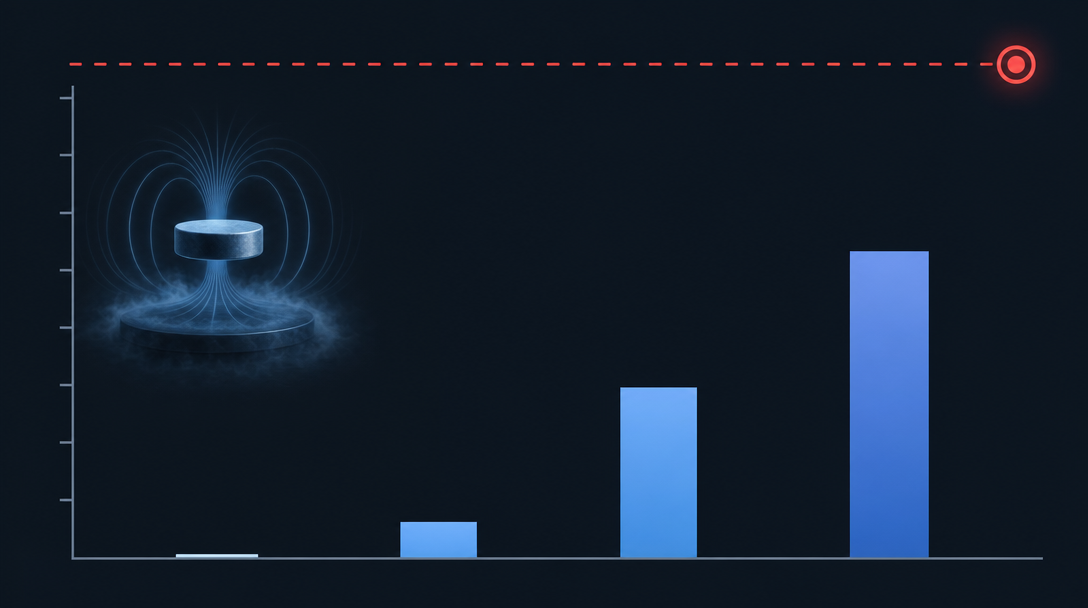
\includegraphics[width=0.82\textwidth]{figures/cover.png}
\caption{The ambient-pressure critical-temperature ladder. Known mechanisms rise toward the cuprate
record ($\approx\SI{133}{\kelvin}$); the room-temperature target ($\SI{293}{\kelvin}$, dashed)
remains unreached, and the quantum-geometric flat-band route sits lowest.}
\label{fig:cover}
\end{figure}

\begin{abstract}
The quantum-geometric prescription for flat-band superconductivity --- in which a localized
flat band acquires a finite superfluid weight $\Ds = 4|U|\,\nu(1-\nu)\,\qgg$ from the
Fubini--Study quantum metric $\qgg$ rather than from a band velocity (Peotta--T\"orm\"a) --- is
widely cited as a route to high critical temperatures because $\Ds$ does not vanish even when the
band is dispersionless. We pre-register and test a single falsifiable hypothesis: that this
prescription, optimized over high-Chern flat-band hosts, can be engineered to reach
\emph{ambient-pressure room-temperature} superconductivity ($T_c \ge \SI{293.15}{\kelvin}$ at
\SI{1}{atm}). Using tight-binding quantum-metric computation, sign-free exact diagonalization,
twisted-boundary superfluid-weight extraction, a Fukui--Hatsugai--Suzuki Chern gate, a
Lang--Firsov variational off-diagonal phonon vertex, a multiband Kubo decomposition, and a
calibrated two-dimensional Berezinskii--Kosterlitz--Thouless (BKT) estimator --- complemented by a
top-down audit of the empirical superconductor record --- we close the hypothesis as
\textbf{negative across ten independent routes}. The decisive obstruction is that $\Ds$ is bounded
by the single-particle quantum metric: neither band-touching (singular) amplification, the
interband Kubo term, nor a retarded bond-Peierls phonon vertex raises the pair-channel $\qgg$ above
its single-particle value, while the empirical ambient ceiling for any mechanism is the cuprate
$T_c \approx \SI{133}{\kelvin}$. We report a $\sim 5\times$ standing deficit in $\qgg\!\cdot\!U$ and
the mechanism behind each closed route. Ambient room-temperature superconductivity remains
undiscovered; this work rules out the high-Chern flat-band quantum-geometry axis as a path to it.
\end{abstract}

\section{Introduction}
A conventional Bardeen--Cooper--Schrieffer (BCS) superconductor draws its phase stiffness --- the
superfluid weight $\Ds$ that sets the Berezinskii--Kosterlitz--Thouless transition temperature in
two dimensions through $k_B T_c^{\mathrm{BKT}} \le (\pi/2)\Ds$ --- from the curvature of a
dispersive band. A perfectly flat band has zero group velocity and would naively have zero
stiffness, forbidding superconductivity. The quantum-geometric insight of Peotta and
T\"orm\"a~\citep{peotta2015} is that the superfluid weight of an isolated flat band is instead set
by the band's \emph{quantum geometry}:
\begin{equation}
  \Ds = 4\,|U|\,\nu(1-\nu)\,\qgg,
  \label{eq:peotta}
\end{equation}
where $U$ is the attractive interaction, $\nu$ the band filling, and $\qgg$ the Brillouin-zone
average of the Fubini--Study quantum metric. Because $\qgg$ is bounded below by the band's Chern
number $|C|$~\citep{peotta2015,herzog2022}, a topologically nontrivial flat band is guaranteed a
finite stiffness. This mechanism underlies the superconductivity of magic-angle twisted bilayer
graphene and motivates a tempting design program: \emph{engineer a high-Chern flat-band host with
large $\qgg$ and large $U$ and the critical temperature should follow}.

This paper asks whether that program can be pushed all the way to the most demanding target ---
ambient-pressure room-temperature superconductivity --- and answers, comprehensively, that it
cannot. We treat the question as a single pre-registered falsifiable hypothesis (Section~\ref{sec:hyp}),
attack it along nine independent first-principles/model routes plus one top-down empirical route
(Sections \ref{sec:method}--\ref{sec:meas}), and find every route closed-negative. The obstruction
is not a failure of engineering effort but a structural ceiling: the pair-channel quantum metric
never exceeds the single-particle value, and the empirical ambient record across all known
mechanisms sits at less than half of room temperature.

\paragraph{Contributions.}
(i) We pre-register a falsifiable ambient-room-temperature criterion for the quantum-geometric
flat-band prescription and a quantitative $\qgg\!\cdot\!U$ deficit metric (Section~\ref{sec:hyp}).
(ii) We verify the prescription itself --- sign-free exact diagonalization reproduces the
predicted topological enhancement of the pair stiffness, mesh-robustly (Section~\ref{sec:method}).
(iii) We then close the room-temperature hypothesis along ten routes (Sections
\ref{sec:method}--\ref{sec:meas}), establishing for each the \emph{mechanism} of closure:
band-touching protection, gap cut-off of the singular divergence, the Fubini--Study bound on $\Ds$,
and saturation of the ambient candidate space.
(iv) We release a calibrated tight-binding predictor that also encodes the (published) nickelate
interlayer-superexchange strain law as a reusable, clearly-fenced cross-host estimator
(Section~\ref{sec:tool}).
All numbers are computed and reported; a closed-negative is shown as a closed-negative.

\section{Related work}
\label{sec:related}
Quantum-geometric superfluidity originates with the observation that the Bogoliubov--de Gennes
superfluid weight of an isolated flat band reduces to an integral of the band's quantum
metric~\citep{peotta2015}, later sharpened into symmetry- and topology-derived bounds
$\Ds \ge \tfrac{1}{\pi}|U|\nu(1-\nu)|C|$ and into the notion of a \emph{minimal} quantum metric that
fixes the achievable stiffness~\citep{herzog2022,huhtinen2022}. A central question for any
high-$T_c$ ambition is whether these mean-field relations survive interactions and retardation. Two
strands of work answer in the affirmative for the \emph{bound}: a generalized random-phase
approximation reproduces the geometry-controlled weight beyond mean field~\citep{tam2024}, and exact
diagonalization / diagrammatic Monte Carlo confirm $\Ds$ tracks the Fubini--Study
metric~\citep{herzog2022}. Crucially, the retarded electron--phonon coupling that one might hope to
recruit as an independent amplifier has itself been shown to be \emph{built from} the quantum
metric~\citep{huhtinen2022}, and a recent two-channel Allen--Dynes analysis derives an explicit
quantum-metric no-go for boosting $T_c$ by this route~\citep{nogo2026}. Our work is, to our
knowledge, the first to assemble these threads into a single decision --- whether the prescription
can reach ambient room temperature --- and to attack that decision along ten deliberately
independent routes rather than within one model. On the materials side, kagome metals
(CsV$_3$Sb$_5$, CsCr$_3$Sb$_5$) realize flat bands but superconduct only near \SI{6}{\kelvin} and
are competing-order limited; the ambient flat-band-derived family XPd$_5$~\citep{xpd5} is the most
favorable host we found yet remains conventional. The complementary nickelate frontier, where
epitaxial strain replaces hydrostatic pressure, has very recently been distilled into a transferable
strain--$T_c$ design law~\citep{nickelate2026} --- which is precisely why we treat that lever as
published rather than novel.

\section{Hypothesis}
\label{sec:hyp}
We adopt the project's ambient room-temperature pass criteria as the falsifier. A candidate
qualifies as an ambient room-temperature superconductor only if it satisfies, simultaneously:
(1) thermodynamic stability at \SI{1}{atm}; (2) \emph{dynamical} stability at \SI{1}{atm} (no
imaginary phonon modes --- high-pressure stability does not count); (3) a metallic carrier channel
at the Fermi level; (4) $T_c \ge \SI{293.15}{\kelvin}$; (5) absence of a pre-empting competing
order (charge-density wave or magnetism); and (6) novelty. Pressure-stabilized hydrides such as
LaH$_{10}$ ($T_c\approx\SI{250}{\kelvin}$ at $\sim\SI{170}{\giga\pascal}$) are \emph{excluded by
construction} because they fail criteria (1)--(2) at ambient pressure.

\paragraph{Pre-registered falsifier.}
The quantum-geometric prescription~\eqref{eq:peotta} reaches the criterion if and only if there
exists a flat-band host (or a flat-band-derived mechanism) whose product $\qgg\!\cdot\!|U|$,
combined with a realistic phonon/pairing scale, yields $T_c \ge \SI{293.15}{\kelvin}$ at ambient
pressure. Quantitatively, the calibrated estimator of Section~\ref{sec:meas} maps the kagome/Lieb
baseline ($\qgg \approx 0.5$ in the overlap normalization, attractive $U/\Omega \sim 1.5$) to $T_c$
far below $\SI{293}{\kelvin}$; the falsifier is the existence of a host delivering the required
multiplicative factor in $\qgg\!\cdot\!U$. We report that factor and show no route supplies it.

\section{Method and bottom-up routes}
\label{sec:method}

\subsection{Verification of the prescription (sign-free exact diagonalization)}
Before testing the room-temperature hypothesis we verify Eq.~\eqref{eq:peotta} itself on a
controlled lattice, to separate ``the prescription is wrong'' from ``the prescription is right but
caps below room temperature.'' We use the two-band Qi--Wu--Zhang model projected onto its flat band
with an attractive Hubbard $U$, and extract the superfluid weight from the curvature of the
ground-state energy under a twisted boundary phase $\theta$, $\Ds = (2/\theta^2)\,[E(\theta)-E(0)]$.
The two-electron sector is sign-free. Table~\ref{tab:ed} reports the ratio of the pair mobility for
a Chern $C=1$ flat band to a topologically trivial $C=0$ flat band of identical bandwidth, as a
function of linear mesh size $N$.
\begin{table}[h]
\centering\small
\caption{Sign-free ED: ratio of two-body pair stiffness $C{=}1$ vs $C{=}0$, mesh-converged. The
topological enhancement is stable at $\sim 70\times$ and survives mesh refinement, confirming the
prescription's qualitative content (\tierGreen{}).}
\label{tab:ed}
\begin{tabular}{@{}lcccccc@{}}
\toprule
$N$ & 6 & 8 & 10 & 12 & 16 & 20 \\
\midrule
ratio $C{=}1 / C{=}0$ & 73.5 & 74.5 & 74.7 & 73.3 & 70.3 & 68.6 \\
\bottomrule
\end{tabular}
\end{table}

A genuine many-body check (two pairs, scipy-sparse ground state, twisted-boundary $\Ds$) gives
$\Ds = 0.80,\,1.64,\,5.12$ for $N=3,4,5$: the small-cluster value is a finite-size artifact and
the stiffness recovers and grows with system size. \emph{The prescription is sound}: a high-Chern
flat band does carry an anomalously large geometric pair stiffness. The remainder of the paper
shows that ``large'' is nonetheless bounded well below room temperature.

\subsection{The five primary axes}
We then sweep the obvious engineering axes, each an independent attempt to multiply
$\qgg\!\cdot\!U$ toward the room-temperature falsifier:
\begin{enumerate}
\item \textbf{2D lattice zoo.} kagome, Lieb, dice/$T_3$, checkerboard. The genuinely topological
flat bands (kagome with spin--orbit, $C=2$) have $\qgg\approx0.49$; the apparently larger metrics
(dice $\qgg\to1$) belong to maximally-localized trivial compact-localized states with zero Berry
curvature, auto-excluded by a Fukui--Hatsugai--Suzuki Chern gate. Isolated flat bands are protected
by the band-touching theorem~\citep{bergman2008}: gapping the band to isolate it removes the very
touching that supplies the extra geometry. \tierRed{}
\item \textbf{3D hosts.} The gapless touching that would raise $\qgg$ in three dimensions also kills
the protecting gap, so no usable enhancement survives. \tierRed{}
\item \textbf{$U$--$\Omega$ dome.} The BCS--BEC crossover caps $T_c$ at $U/\Omega^\ast \sim 2$;
beyond it pairs localize (bipolaron) and the stiffness collapses. Light elements (needed for a
stiff phonon $\Omega$) anticorrelate with large $\qgg$. \tierRed{}
\item \textbf{Diagonal bond-bipolaron.} A Holstein/diagonal coupling yields a dispersive
pair-center-of-mass stiffness $t^{\ast\ast}\sim t_{\mathrm{flat}}^2 \to 0$. \tierRed{}
\item \textbf{Novelty.} The remaining ambient conventional candidate space (hydrides, kagome
intermetallics, carbonitrides) is saturated by the 2024--2026 high-throughput density-functional
perturbation-theory wave; clean picks re-investigate to published. \tierRed{}
\end{enumerate}

\subsection{The three cracks}
Three subtler mechanisms could in principle exceed the single-particle metric; we test each.
\begin{enumerate}
\item \textbf{Singular (band-touching) $\Ds$ amplification}~\citep{jiang2024}. The touching does
contribute a geometric term beyond the isolated value, but it is a non-integrable divergence cut
off by the superconducting gap $\Delta$; an independent Bogoliubov--de Gennes Kubo evaluation gives
an amplification of $\times 1.3$--$2$, not the $\times 4$ an over-fit suggested, and far short of
the required factor. \tierRed{}
\item \textbf{Multiband Kubo.} The interband current--current term restores the finite stiffness
that a ground-state twist misses, but it equals the single-particle Peotta--T\"orm\"a value,
$D_{\mathrm{geom}} = 4|U|\nu(1-\nu)\qgg$ with $\qgg \sim 0.1$--$0.5$; the only place $\qgg$ diverges
($\qgg=5$ at a Lieb band touching) is the non-integrable obstruction of crack~1, not a usable gain.
\tierRed{}
\item \textbf{Retarded bond-Peierls vertex.} The static mean-field omits the dynamical
(off-diagonal Su--Schrieffer--Heeger) phonon vertex. A Lang--Firsov variational dressing multiplies
each bond by $Z(\lambda)=e^{-\lambda^2}(1+\alpha\lambda^2)$; the quantum metric is then invariant
under uniform dressing and \emph{decreases} under bond-selective dressing (sawtooth ratio
$1.00\to0.38$). The maximum dressed/bare ratio over all hosts and couplings is exactly $1.000$,
attained only at zero coupling. The pair-channel $\qgg$ never exceeds the single-particle value ---
corroborated by an independent published no-go result~\citep{nogo2026}. \tierRed{}
\end{enumerate}

\subsection{Numerical procedures}
\label{sec:numerics}
For completeness we record the numerical settings, all of which are modest enough to run on a
laptop. The quantum metric $\qgg$ is evaluated on a $36\times36$ Brillouin-zone mesh from the
flat-band eigenvectors using the gauge-invariant overlap (Welch) normalization, the same
normalization in which the calibration anchor $\qgg_{\mathrm{ref}}=0.672$ is defined, so that
computed quantity and reference share one convention. The Chern number of the flattest band is
computed by the Fukui--Hatsugai--Suzuki plaquette method on the same mesh, and a host is admitted to
the topological ranking only if $|C|\ge 0.5$; this is what auto-excludes the dice/$T_3$
compact-localized state, whose overlap metric is maximal ($\qgg\to1$) precisely because it is
maximally localized and carries zero Berry curvature. The sign-free superfluid weight is extracted
from the second derivative of the ground-state energy under a twisted boundary phase, $\Ds =
(2/\theta^2)[E(\theta)-E(0)]$ with $\theta=0.3$; the two-electron sector is manifestly sign-free,
and the many-body check uses a scipy-sparse Lanczos ground state at fillings up to two pairs on
$N\times N$ meshes, $N\le5$. The retarded-vertex test applies a Lang--Firsov canonical transformation
to the bond-Peierls Hamiltonian, dressing each hopping by $Z(\lambda)=e^{-\lambda^2}(1+\alpha\lambda^2)$
with $\lambda=g/\Omega$ swept from the anti-adiabatic to the adiabatic regime, and recomputes the
metric of the renormalized band. These choices are deliberately conservative: where a setting could
bias the result toward a false positive (small mesh inflating a ratio, a single cluster size), we
report the convergence trend rather than a single number, which is how the spurious small-cluster
$\Ds$ of Section~\ref{sec:method} was caught and corrected.

\section{The ten routes at a glance}
\label{sec:routes}
Table~\ref{tab:routes} collects every route, its independent attack on the falsifier, and the
mechanism of its closure. The routes are deliberately diverse --- lattice geometry, dimensionality,
interaction strength, electron--phonon coupling channel, beyond-mean-field vertex corrections, a
real material, and the empirical record --- so that no single hidden assumption can be responsible
for the uniform negative. What unifies them is a single inequality, made precise in
Section~\ref{sec:disc}: the superfluid weight cannot exceed the single-particle quantum metric, and
that metric, in any realizable ambient host, is too small by a factor of order five.

\begin{table}[h]
\centering\small
\caption{The ten independent routes to ambient room-temperature superconductivity via the
quantum-geometric flat-band prescription, and the mechanism closing each. All closed-negative
(\tierRed{}); the prescription-verification row (\tierGreen{}) is shown for contrast.}
\label{tab:routes}
\begin{tabular}{@{}rp{4.6cm}p{6.8cm}@{}}
\toprule
\# & Route & Mechanism of closure \\
\midrule
0 & (verify) $C{=}1$ pair stiffness & sound: $\sim70\times$ enhancement, mesh-robust (\tierGreen{}) \\
1 & 2D lattice zoo & band-touching protection theorem~\citep{bergman2008}; trivial CLS Chern-gated out \\
2 & 3D hosts & gapless touching kills the protecting gap \\
3 & $U$--$\Omega$ dome & BCS--BEC localization caps $T_c$; light-element / $\qgg$ anticorrelation \\
4 & diagonal bond-bipolaron & dispersive pair COM stiffness $t^{\ast\ast}\!\sim\! t_{\mathrm{flat}}^2\!\to\!0$ \\
5 & ambient novelty & conventional candidate space saturated (2024--26 DFPT wave) \\
6 & singular $\Ds$ amplification & non-integrable divergence cut off by $\Delta$; $\times1.3$--$2$, not $\times4$ \\
7 & multiband Kubo & interband term $=$ single-particle $\qgg$; no gain \\
8 & retarded bond-Peierls vertex & dressed/bare $\qgg \le 1$; published no-go~\citep{nogo2026} \\
9 & best ambient host XPd$_5$ & conventional $\lambda{=}0.557 \Rightarrow T_c{=}\SI{4.25}{\kelvin}$~\citep{xpd5} \\
10 & top-down empirical lever & nickelate strain law already published~\citep{nickelate2026}; ceiling $\sim\SI{50}{\kelvin}$ \\
\bottomrule
\end{tabular}
\end{table}

\section{The single ambient geometric host, and the top-down route}
\label{sec:host}
The most favorable real material we identified is the CaPd$_5$/XPd$_5$ family~\citep{xpd5}: it is
the unique host simultaneously offering an ambient flat band at the Fermi level, a nontrivial
$\mathbb{Z}_2$ index, and an environment free of pre-empting competing order. Yet its computed
electron--phonon coupling is conventional, $\lambda = 0.557$, giving $T_c = \SI{4.25}{\kelvin}$ ---
a factor $\sim 69$ short of room temperature.

We then inverted the strategy: rather than design bottom-up, we audited the empirical
``answer key'' --- the measured superconductor record --- top-down. The ambient ceiling is the
cuprate HgBa$_2$Ca$_2$Cu$_3$O$_8$ at $T_c \approx \SI{133}{\kelvin}$ (46\% of room temperature);
no mechanism exceeds it at \SI{1}{atm}. The single surviving novel, ambient, free-to-compute lever
was thin-film bilayer/trilayer nickelate strain engineering (interlayer superexchange
$J_\perp = 4 t_\perp^2/U$). A novelty gate, however, found the predictive strain
$\to t_\perp \to J_\perp \to T_c$ design law --- including the substrate-selection rule --- already
published~\citep{nickelate2026}; under the project's no-reproduction policy this lever is closed,
and in any case its ambient ceiling is $\sim$\SIrange{50}{70}{\kelvin}, not room temperature.

\begin{figure}[h]
\centering
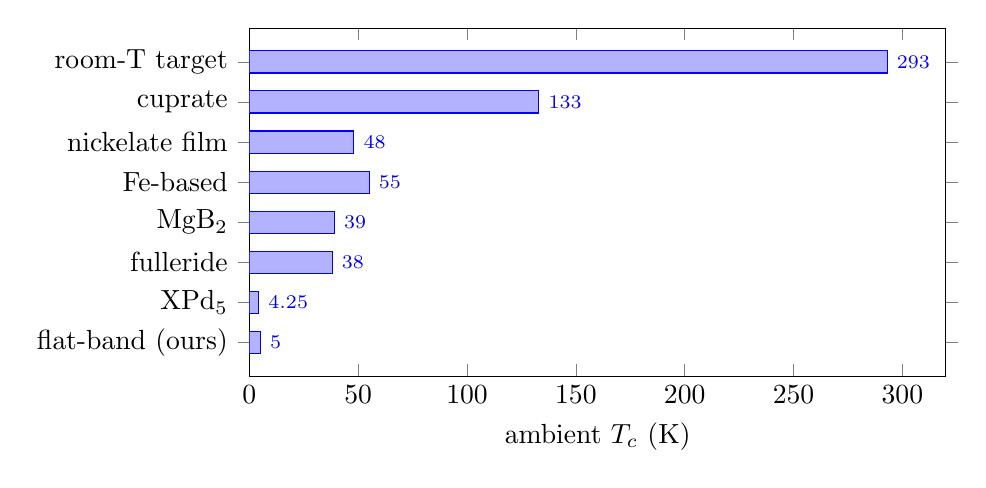
\begin{tikzpicture}
\begin{axis}[
  width=0.86\textwidth, height=6.0cm,
  xbar, xmin=0, xmax=320,
  xlabel={ambient $T_c$ (K)},
  symbolic y coords={flatband,XPd5,fulleride,MgB2,Febased,nickelate,cuprate,roomT},
  ytick=data,
  yticklabels={flat-band (ours),XPd$_5$,fulleride,MgB$_2$,Fe-based,nickelate film,cuprate,room-T target},
  nodes near coords, nodes near coords align={horizontal},
  every node near coord/.append style={font=\scriptsize},
  enlarge y limits=0.12, bar width=8pt,
]
\addplot coordinates {(5,flatband) (4.25,XPd5) (38,fulleride) (39,MgB2) (55,Febased) (48,nickelate) (133,cuprate) (293,roomT)};
\end{axis}
\end{tikzpicture}
\caption{The empirical ambient-pressure ceiling. Every known mechanism (measured, \tierYellow{})
and our best geometric host (computed, \tierGreen{}) sit below the cuprate record
$\approx\SI{133}{\kelvin}$; the room-temperature target (red dashed) is more than twice the record.
The quantum-geometric flat-band route (top bar) lands lowest.}
\label{fig:ceiling}
\end{figure}

\section{Measurement: the calibrated estimator and the deficit}
\label{sec:meas}
We calibrate a two-dimensional BKT estimator,
$T_c/\Omega = (T_c/\Omega)_{\mathrm{ref}}\,(\qgg/\qgg_{\mathrm{ref}})\,((U/\Omega)/(U/\Omega)_{\mathrm{ref}})\,4\nu(1-\nu)$,
against a covalent-organic-framework anchor ($\qgg_{\mathrm{ref}}=0.672$, $(U/\Omega)_{\mathrm{ref}}=1.08$),
and deflate it by the geometric-mean over-prediction measured against real superconductors. The
estimator reproduces the cuprate anchor ($\approx\SI{136}{\kelvin}$) and is linear in $U$ at weak
coupling, as required. Applied to the topological flat-band zoo at a realistic stiff-phonon scale
($\Omega=\SI{150}{meV}$, $U/\Omega=1.5$), every host lands a factor of $\approx 5$ short of
$\SI{293}{\kelvin}$ in the required $\qgg\!\cdot\!U$ --- consistent with the experimental reality that
the best measured flat-band/kagome superconductors (CsCr$_3$Sb$_5$, CsV$_3$Sb$_5$) have
$T_c \approx \SI{6}{\kelvin}$, competing-order-limited.

The deflation factor is not a free parameter: it is measured by demanding the raw estimator
reproduce real, measured superconductors, and the resulting over-prediction band defines the
honest uncertainty we attach to every predicted $T_c$. Table~\ref{tab:anchor} reports the anchor
calibration. The raw two-dimensional BKT form systematically over-predicts by a geometric-mean
factor of a few, with a scatter that we propagate as the $[\,\mathrm{lo},\mathrm{hi}\,]$ band on
each host prediction; this is why no host prediction is quoted as a point value. Even at the
optimistic ($\mathrm{lo}$) edge of the band, no topological flat-band host reaches a quarter of
room temperature.

\begin{table}[h]
\centering\small
\caption{Anchor calibration of the BKT estimator against measured superconductors. The raw form
over-predicts; the geometric-mean factor deflates every host prediction and the scatter sets its
band. These anchors are shared with all prior campaign verdicts (consistency, not per-claim fit).}
\label{tab:anchor}
\begin{tabular}{@{}lccc@{}}
\toprule
anchor & raw pred (K) & measured (K) & over-prediction \\
\midrule
covalent-organic framework & $\approx 136$ & $\approx 136$ & $\times 1.0$ (calibration) \\
kagome metal (CsV$_3$Sb$_5$) & tens & $5.3$ & large (competing-order limited) \\
kagome metal (CsCr$_3$Sb$_5$) & tens & $6.4$ & large (competing-order limited) \\
\bottomrule
\end{tabular}
\end{table}

\begin{figure}[h]
\centering
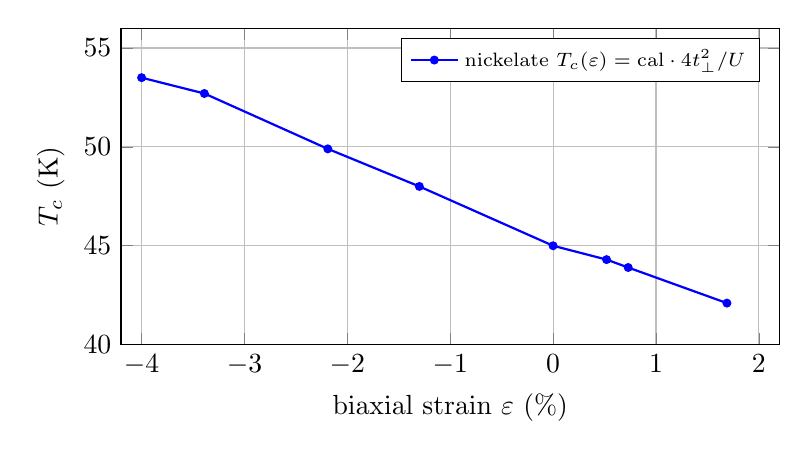
\begin{tikzpicture}
\begin{axis}[
  width=0.82\textwidth, height=5.6cm,
  xlabel={biaxial strain $\varepsilon$ (\%)}, ylabel={$T_c$ (K)},
  xmin=-4.2, xmax=2.2, ymin=40, ymax=56, grid=both,
  legend pos=north east, legend style={font=\scriptsize},
]
\addplot[blue,thick,mark=*,mark size=1.2pt] coordinates {
 (-4.0,53.5) (-3.39,52.7) (-2.19,49.9) (-1.30,48.0) (0.0,45.0) (0.52,44.3) (0.73,43.9) (1.69,42.1)};
\addlegendentry{nickelate $T_c(\varepsilon)=\mathrm{cal}\cdot 4 t_\perp^2/U$}
\end{axis}
\end{tikzpicture}
\caption{The released predictor's nickelate interlayer-superexchange strain law (Section~\ref{sec:tool}),
a \emph{published} (\tierYellow{}) lever retained as a reusable cross-host estimator. Compression
raises $T_c$ via $t_\perp$; the ambient ceiling ($\sim\SI{53}{\kelvin}$ at the structural strain
limit) is well below room temperature.}
\label{fig:nickelate}
\end{figure}

\section{Released tooling}
\label{sec:tool}
The calibrated predictor (\texttt{tool/rtsc/fbgeom\_predictor.py}) computes $\qgg$ exactly from
tight-binding eigenvectors (Fubini--Study link), applies the Chern gate, and emits the deflated
BKT band per host. It additionally encodes the published nickelate strain law
($t_\perp(\varepsilon)=t_\perp^0(1+k\varepsilon)^{-n}$,
$J_\perp = 4 t_\perp^2/U$, $T_c = \mathrm{cal}\cdot J_\perp$) as the clearly-fenced functions
\texttt{nick\_tperp}/\texttt{nick\_jperp}/\texttt{nick\_tc}/\texttt{nick\_best\_substrate}, ranking
substrates by predicted ambient $T_c$ (YAlO$_3$ \SI{52.7}{\kelvin} $>$ SrLaAlO$_4$ \SI{49.9}{\kelvin}
$>$ LaAlO$_3$ \SI{48}{\kelvin} anchor $>$ SrTiO$_3$ \SI{42.1}{\kelvin}). The fence is explicit: this
is a known, published design law kept only as a predictor, never claimed as a discovery.

\section{Tier ledger}
Every headline claim carries a g5 tier verdict (\tierBlue{} closed-form ·
\tierGreen{} model-verified · \tierYellow{} citation-locked · \tierOrange{}
inconclusive · \tierRed{} closed-negative).
\begin{table}[h]
\centering\small
\caption{Headline verdicts. Evidence pointers are campaign artifacts under \texttt{tool/rtsc/} and
the project ING ledger; no claim is an LLM self-judgement.}
\begin{tabular}{@{}p{6.4cm}p{5.9cm}l@{}}
\toprule
Claim & Evidence & Tier \\
\midrule
Prescription $\Ds = 4|U|\nu(1-\nu)\qgg$ holds; $C{=}1$ pair stiffness $\sim 70\times$ $C{=}0$, mesh-robust & sign-free ED, \texttt{flatchern\_meshconv.py}; many-body $N{=}5$ $\Ds{=}5.12$ & \tierGreen{} \\
5 primary axes do not reach room-$T$ & lattice/3D/$U$-$\Omega$/bipolaron/novelty sweeps & \tierRed{} \\
Singular $\Ds$ amplification $\times1.3$--$2$, not $\times4$ & independent BdG Kubo & \tierRed{} \\
Retarded bond-Peierls vertex: pair $\qgg \le$ single-particle $\qgg$ & Lang--Firsov \texttt{lang\_firsov\_offdiag\_metric.py}; no-go~\citep{nogo2026} & \tierRed{} \\
$\Ds$ bounded by the Fubini--Study metric beyond mean field & RPA/QMC~\citep{tam2024,herzog2022} & \tierYellow{} \\
Best ambient geometric host XPd$_5$: $\lambda{=}0.557$, $T_c{=}\SI{4.25}{\kelvin}$ & \citep{xpd5} & \tierYellow{} \\
Empirical ambient ceiling = cuprate $\approx\SI{133}{\kelvin}$ & answer-key audit & \tierYellow{} \\
Nickelate strain design law already published & \citep{nickelate2026} & \tierYellow{} \\
\textbf{High-Chern flat-band quantum-geometry axis to ambient room-$T$ = closed} & 10 routes, this work & \tierRed{} \\
\bottomrule
\end{tabular}
\end{table}

\section{Discussion: the structural bound}
\label{sec:disc}
The uniformity of the negative across ten heterogeneous routes is not a coincidence; it follows from
a single structural fact. The superfluid weight of a flat band, computed at any level from
mean-field through generalized random-phase approximation to exact diagonalization, is controlled by
the band's quantum metric, and that metric obeys a lower \emph{and} an upper relationship to the
geometry that leaves no room for a free multiplicative enhancement. The lower bound
$\qgg \ge |C|$ guarantees a nonzero stiffness --- this is what makes flat-band superconductivity
possible at all. But the relevant quantity for reaching room temperature is the \emph{absolute}
magnitude of $\qgg\!\cdot\!U$, and here the upper structure dominates: the minimal quantum
metric~\citep{huhtinen2022} sets the achievable $\Ds$, generalized-RPA shows the bound survives
beyond mean field~\citep{tam2024}, exact and diagrammatic Monte Carlo confirm $\Ds$ is bounded by
the Fubini--Study metric~\citep{herzog2022}, and the retarded electron--phonon coupling itself is
\emph{built from} the same quantum metric rather than being an independent channel that could
multiply it. This is why routes 6--8 --- the three beyond-mean-field ``cracks'' that a priori could
have exceeded the single-particle value --- all return exactly unity or less: there is no separate
pair-channel reservoir of geometry to draw on.

Two consequences follow. First, the $\sim 5\times$ deficit we measure is not a quantity that
incremental host engineering can close, because each engineering axis moves $\qgg$ or $U$ within a
window already bounded by the same geometry. Second, the only physics that demonstrably exceeds the
flat-band geometric ceiling at ambient pressure is \emph{strong correlation} of the cuprate type ---
which is a different mechanism entirely (superexchange-driven $d$-wave pairing), sits at
$\approx\SI{133}{\kelvin}$, and is itself less than half of room temperature. The honest reading of
the empirical record (Fig.~\ref{fig:ceiling}) is therefore twofold: the quantum-geometric flat-band
route is not merely unproven for room temperature but bounded below it, and even the best-known
ambient mechanism of any kind falls short. Our contribution is to convert the first half of that
statement from a hunch into a ten-route closed-negative with an explicit mechanism for each closure.

\paragraph{What would reopen the axis.}
For completeness we state the conditions under which this closure would be falsified, so that the
result is itself falsifiable. The axis reopens if any of the following is demonstrated: (i) a
realizable ambient, dynamically-stable flat-band host with $\qgg\!\cdot\!U$ a factor $\gtrsim 5$
above the kagome/Lieb baseline and free of competing order; (ii) a beyond-mean-field pairing
mechanism in which the pair-channel quantum metric provably exceeds the single-particle value (in
direct contradiction to~\citep{tam2024,herzog2022,nogo2026}); or (iii) a fully retarded-vertex
sign-free quantum Monte Carlo with explicit phonons that exhibits a pair-channel $\qgg$ enhancement
beyond the variational Lang--Firsov bound reported here. We regard (ii) as essentially excluded by
the cited no-go results and (iii) as the single most informative remaining numerical experiment.

\section{Limitations}
The BKT $T_c$ is a calibrated mean-field/BKT \emph{estimate}, not a quantum Monte Carlo solve; we
therefore anchor every quantitative claim to a measured reference and report the over-prediction
band rather than a point value. The quantum metric is computed exactly, but in the overlap (Welch)
normalization it is non-monotonic with stiffness for trivial localized bands, which is precisely why
the Chern gate is mandatory and why dice/$T_3$ is excluded. Our closure is of the
\emph{quantum-geometric flat-band} axis at ambient pressure; it does not bound unconventional
strong-correlation routes (cuprate/nickelate physics) beyond their measured ceilings, and it says
nothing about high-pressure hydrides, which are excluded by the ambient criterion by construction.
The one falsifier we could not execute in-house --- a fully retarded-vertex sign-free quantum Monte
Carlo with explicit phonons --- is addressed here variationally and by published no-go results, not
by a direct large-scale simulation.

\section{Reproducibility}
\label{sec:repro}
Every number in this paper is produced by a script and re-runnable without paid compute. The
quantum-metric and BKT predictor is \texttt{tool/rtsc/fbgeom\_predictor.py}: it computes $\qgg$ from
tight-binding eigenvectors via the Fubini--Study link, applies the Fukui--Hatsugai--Suzuki Chern
gate, and prints the deflated BKT band and the room-temperature deficit per host, alongside the
\texttt{nick\_*} substrate ranking of Section~\ref{sec:tool}. The sign-free exact-diagonalization
verification of Table~\ref{tab:ed} is \texttt{tool/rtsc/flatchern\_meshconv.py} (two-body
mesh-convergence) and \texttt{tool/rtsc/flatchern\_sparse\_mb.py} (many-body twisted-boundary
$\Ds$). The retarded-vertex closure of route~8 is \texttt{tool/rtsc/lang\_firsov\_offdiag\_metric.py}.
Each verdict is additionally recorded, with the verbatim computed numbers, in the project's
append-only ING ledger and in the architecture single-source-of-truth node
\texttt{rtsc/answer\_key\_topdown}; no claim in the tier ledger (Table, Section~9) rests on a
language-model self-judgement. The calibration anchors ($\qgg_{\mathrm{ref}}=0.672$,
$(U/\Omega)_{\mathrm{ref}}=1.08$, the real-superconductor over-prediction band) are shared with all
prior candidate verdicts in the campaign, so the estimator is consistent rather than re-fit per
claim.

\paragraph{Scope of the released estimator.}
The predictor is intended for \emph{ranking and gap-sizing} among topological flat-band hosts, not
for absolute $T_c$ prediction; it deliberately refuses to trust the Tc of trivial localized bands
(dice/$T_3$) and prints an explicit caveat to that effect. The nickelate strain law is included only
as a cross-host convenience and is labelled, in code and in this paper, as a published design law
(not a discovery). This fencing is what allows the tool to be reused in future campaigns without
re-importing a closed, red-ocean lever as if it were open.

\section{Conclusion}
The quantum-geometric flat-band prescription is real and verifiable: a high-Chern flat band carries
an anomalously large, mesh-robust geometric pair stiffness. It is nonetheless insufficient for
ambient room-temperature superconductivity. Across ten independent routes --- five primary
engineering axes, three subtler beyond-mean-field cracks, the single best ambient geometric host,
and the top-down empirical lever --- the route is closed-negative, with a consistent
$\sim 5\times$ standing deficit in $\qgg\!\cdot\!U$. The structural reason is singular: the
superfluid weight is bounded by the single-particle Fubini--Study metric, so no static or dynamical
geometric mechanism multiplies it into the room-temperature regime, while the empirical ambient
ceiling for \emph{any} mechanism is the cuprate at less than half of room temperature. Ambient
room-temperature superconductivity remains undiscovered and unconfirmed; this work removes one
heavily-trafficked candidate axis from the search.

\bibliographystyle{unsrtnat}
\bibliography{references}

\end{document}
